\section{Spontaneous relaxation. Weisskopf-Wigner theory}

We have shown that excited two-level atom can perform transitions from the upper state to the lower state and vice versa even \textit{without} external field. Intuitively clear that such process cannot last forever and experiments prove this idea. In our model before we did not have such relaxation process because we take in account only one mode of field (we neglected the continuum of modes in \eqref{eq:hamillll}). Fir a proper account of the atomic decay a continuum of modes, corresponding to a quantization cavity which is infinite in extent, needs to be included.

\begin{figure}[h!]
	\centering
	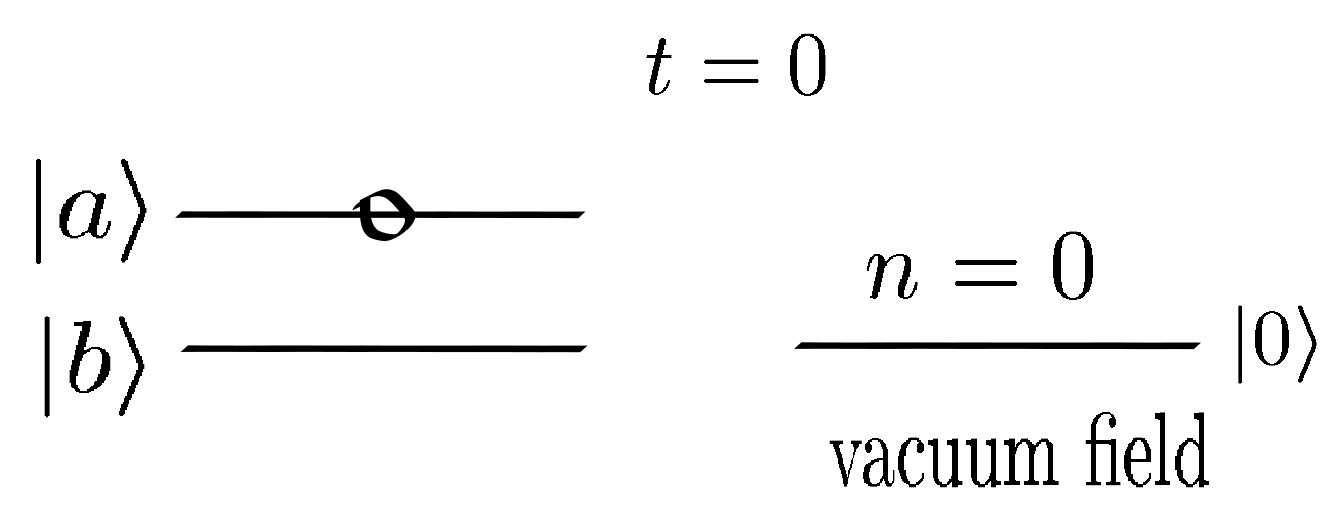
\includegraphics[width=0.5\linewidth]{fig/L7/1}
	\caption{Initial conditions}
	\label{fig:1}
\end{figure}

In other words we consider a two-level system in a huge box with linear dimension $L$ with quantized electromagnetic field inside.
The \textit{interaction picture} Hamiltonian, in the rotating-wave approximation, for this system is
\begin{equation}
	\hat{V}(t) = \hbar \sum_{\kv} \left[ g_{\kv}^* \hat{\sigma}_+ \hat{a}_{\kv} e^{i(\omega_0 - \omega_{\kv})t} + H.c. \right].
\end{equation}
We want to study the system dynamics. Wave functions
\begin{equation}
\ket{\psi(t)} = \sum_{n, \kv} \left( c_{a, n_{\kv}}(t) \ket{a} \ket{n_{\kv}} + c_{b, n_{\kv}}(t) \ket{b} \ket{n_{\kv}} \right),
\end{equation}
where $c_{a(b),n_{\kv}} \myeq c_{a(b), n_{\kv_1}, n_{\kv_2}, \dots}$ and $\ket{n_{\kv}} \myeq \ket{n_{\kv_1}} \ket{n_{\kv_2}} \cdot \dots$. We assume that at time $t=0$ the atom is in the excited state $\ket{a}$ and the field modes are in the vacuum state $\ket{0}$. The state vector is therefore: 
\begin{equation}
	\ket{\psi(t)} = c_{a,0}(t) \ket{a}\ket{0} + \sum_{\kv} c_{b, \kv}(t) \ket{b}\ket{1_{\kv}}, 
\end{equation}
which satisfies the interaction picture Schroedinger equation 
\begin{equation}
i \hbar \ket{\dot{\psi}(t)} = \hat{V}(t) \ket{\psi(t)}
\end{equation}
with initial conditions
\begin{equation}
	c_{a,0}(0) = 1, \qquad c_{b,\kv}(0) = 0.
\end{equation}

From the Schroedinger equation we get the equations of motion for the probability amplitudes:
\begin{subnumcases}{}
	\dot{c}_{a,0} (t) = -i \sum_{\kv} g_{\kv}^* e^{i \Delta_{\kv}t} c_{b,1_{\kv}}(t), \label{eq:7.6a} \\
	\dot{c}_{b,1_{\kv}} (t) = -i g_{\kv} e^{-i\Delta_{\kv}t} c_{a,0}(t), \label{eq:7.6b}
\end{subnumcases}
where $\Delta_{\kv} \myeq  \omega_0 - \omega_{\kv}$. To solve this system we, at first, $\int \eqref{eq:7.6b} dt$:
\begin{equation}
	c_{b,1_{\kv}} (t) = -i g_{\kv} \int \limits_{0}^{t} d \tau e^{-i \Delta_{\kv} \tau} c_{a,0}(\tau).
	\label{eq:tmpppppppp}
\end{equation}
After that we substitute \eqref{eq:tmpppppppp} to \eqref{eq:7.6a} and get the differential-integral equation
\begin{equation}
	\dot{c}_{a,0} (t) = - \sum_{\kv} \left| g_{\kv} \right|^2  \int \limits_0^t d \tau e^{-i \Delta_{\kv} (\tau - t)} c_{a,0}(\tau).
	\label{eq:77777}
\end{equation}
This is still an exact equation. Next shall we make some approximations.

Assuming that the modes of the field are closely spaced in frequency, we can
\begin{equation}
	\sum_{\kv} \qquad \overset{L\to \infty}{\longrightarrow} \qquad 2 \cdot V \int \frac{d^3 k}{(2 \pi)^3}
\end{equation}
where factor $2$ is from averaging over polarization and $\int d^3k = \int_{0}^{\infty} k^2 dk \int_{0}^{2 \pi} d\varphi  \int_{0}^{\pi} \sin \vartheta d \vartheta$ in spherical coordinate system. We remind that $g_{\kv} = - (\vec{d} \cdot \bm{\varepsilon}_{\kv}) / \hbar$ --- coupling constant between the atom and $\kv$-mode. System has a preferred direction: $\vec{d}$. Shall we write it explicitly
\begin{equation}
	g_{\kv} = - \frac{d \varepsilon_{\kv}}{\hbar} \cos \vartheta.
\end{equation}
This allows us easily integrate over $\vartheta$ and $\varphi$:
\begin{equation}
	\int \limits_{0}^{2 \pi} \int \limits_{0}^{\pi} \left| g_{\kv} \right|^2 \sin \vartheta d \varphi d \vartheta = \frac{\left(|\vec{d}| \varepsilon_{\kv}\right)^2}{\hbar^2} \cdot 2 \pi \int \limits_{0}^{\pi} d \vartheta \cos^2 \vartheta \sin \vartheta =  \frac{\left(|\vec{d}| \varepsilon_{\kv}\right)^2}{\hbar^2} \cdot \frac{4 \pi}{3}.
\end{equation}
It means that \eqref{eq:77777} becomes
\begin{equation}
	\dot{c}_{a,0} (t) = - \frac{2 V}{(2\pi \hbar)^3} \cdot \frac{4 \pi}{3} |\vec{d}|^2 \int \limits_{0}^{\infty} dk \int \limits_{0}^{t} d \tau k^2 \varepsilon_{\kv}^2 e^{-i \Delta_{\kv} (\tau - t)} c_{a,0}(\tau).
\end{equation}
Now shall we rewrite the $\int dk$ part using dispersion law $k = \omega_{\kv}/c$ and reminding that $\varepsilon_{\kv}^2 = \frac{\hbar \omega_{\kv}}{2 \varepsilon_0 V}$ (it comes from the expansion of electric field in ladder operators):
\begin{equation}
	\int \limits_{0}^{\infty} dk k^2 \frac{\hbar \omega_{\kv}}{2 \varepsilon_0 V} e^{-i \Delta_{\kv} (\tau - t)} = \frac{\hbar}{2 c^3 \varepsilon_0 V} \int \limits_0^{\infty} d \omega_{\kv} \omega_{\kv}^3 e^{-i (\omega_0 - \omega_{\kv})(\tau - t)},
\end{equation}
so
\begin{equation}
	\dot{c}_{a,0} (t) = - \frac{2 V}{(2\pi \hbar)^3} \cdot \frac{4 \pi}{3} |\vec{d}|^2 \cdot \frac{\hbar}{2 c^3 \varepsilon_0 V} \int \limits_{0}^{\infty} d \omega_{\kv} \int \limits_{0}^{t} d \tau \omega_{\kv}^3 e^{-i (\omega_0 - \omega_{\kv})(\tau - t)} c_{a,0}(\tau).
\end{equation}
In the emission spectrum, the intensity of light associated with the emitted radiation is going to be centered about the atomic transition frequency $\omega_0$. The quantity $\omega_{\kv}^3$ varies little around $\omega_{\kv} = \omega_0$ for which the time integral is not negligible. 
\begin{otherlanguage}{russian}	
\textcolor{red}{Что-то здесь мутный переход, мне не совсем понятно всё. Кстати, график подынтегрального выражения, что у Вас в конспекте в этом месте неверный, так не получится, если построить.}
\end{otherlanguage}
Therefore here we can use the \textit{stationary-phase method}:
\begin{equation}
	\int \limits_{0}^{\infty} d \omega_{\kv}  \omega_{\kv}^3 e^{-i (\omega_0 - \omega_{\kv})(\tau - t)} \quad \to \quad \omega_{0}^3 \int \limits_{-\infty}^{\infty} d \omega_{\kv} e^{-i (\omega_0 - \omega_{\kv})(\tau - t)} = \omega_{0}^3 \cdot 2 \pi \delta(\tau - t).
\end{equation}
Now integral over $d \tau$ is easy to take $\int_0^t d \tau \delta(\tau - t) c_{a,0}(\tau) = \frac{1}{2} c_{a,0}(t)$ and we finally obtain
\begin{equation}
	\dot{c}_{a,0} (t) = - \frac{\gamma}{2} c_{a,0} (t), \qquad \to \qquad c_{a,0}(t) = \exp \left[- \frac{\gamma}{2} t \right],
\end{equation}
where the \textit{decay constant}
\begin{equation}
	\gamma \myeq \frac{\omega_{0}^3 |\vec{d}|^2}{3 \pi \hbar c^3 \varepsilon_0}.
\end{equation}
If we consider a medium which effectively change the wave vector  $k \to nk$ with refractive index $n$ then we get
\begin{equation}
	\gamma = \frac{\omega_{0}^3 |\vec{d}|^2 n}{3 \pi \hbar c^3 \varepsilon_0}.
\end{equation}
\begin{figure}
	\centering
	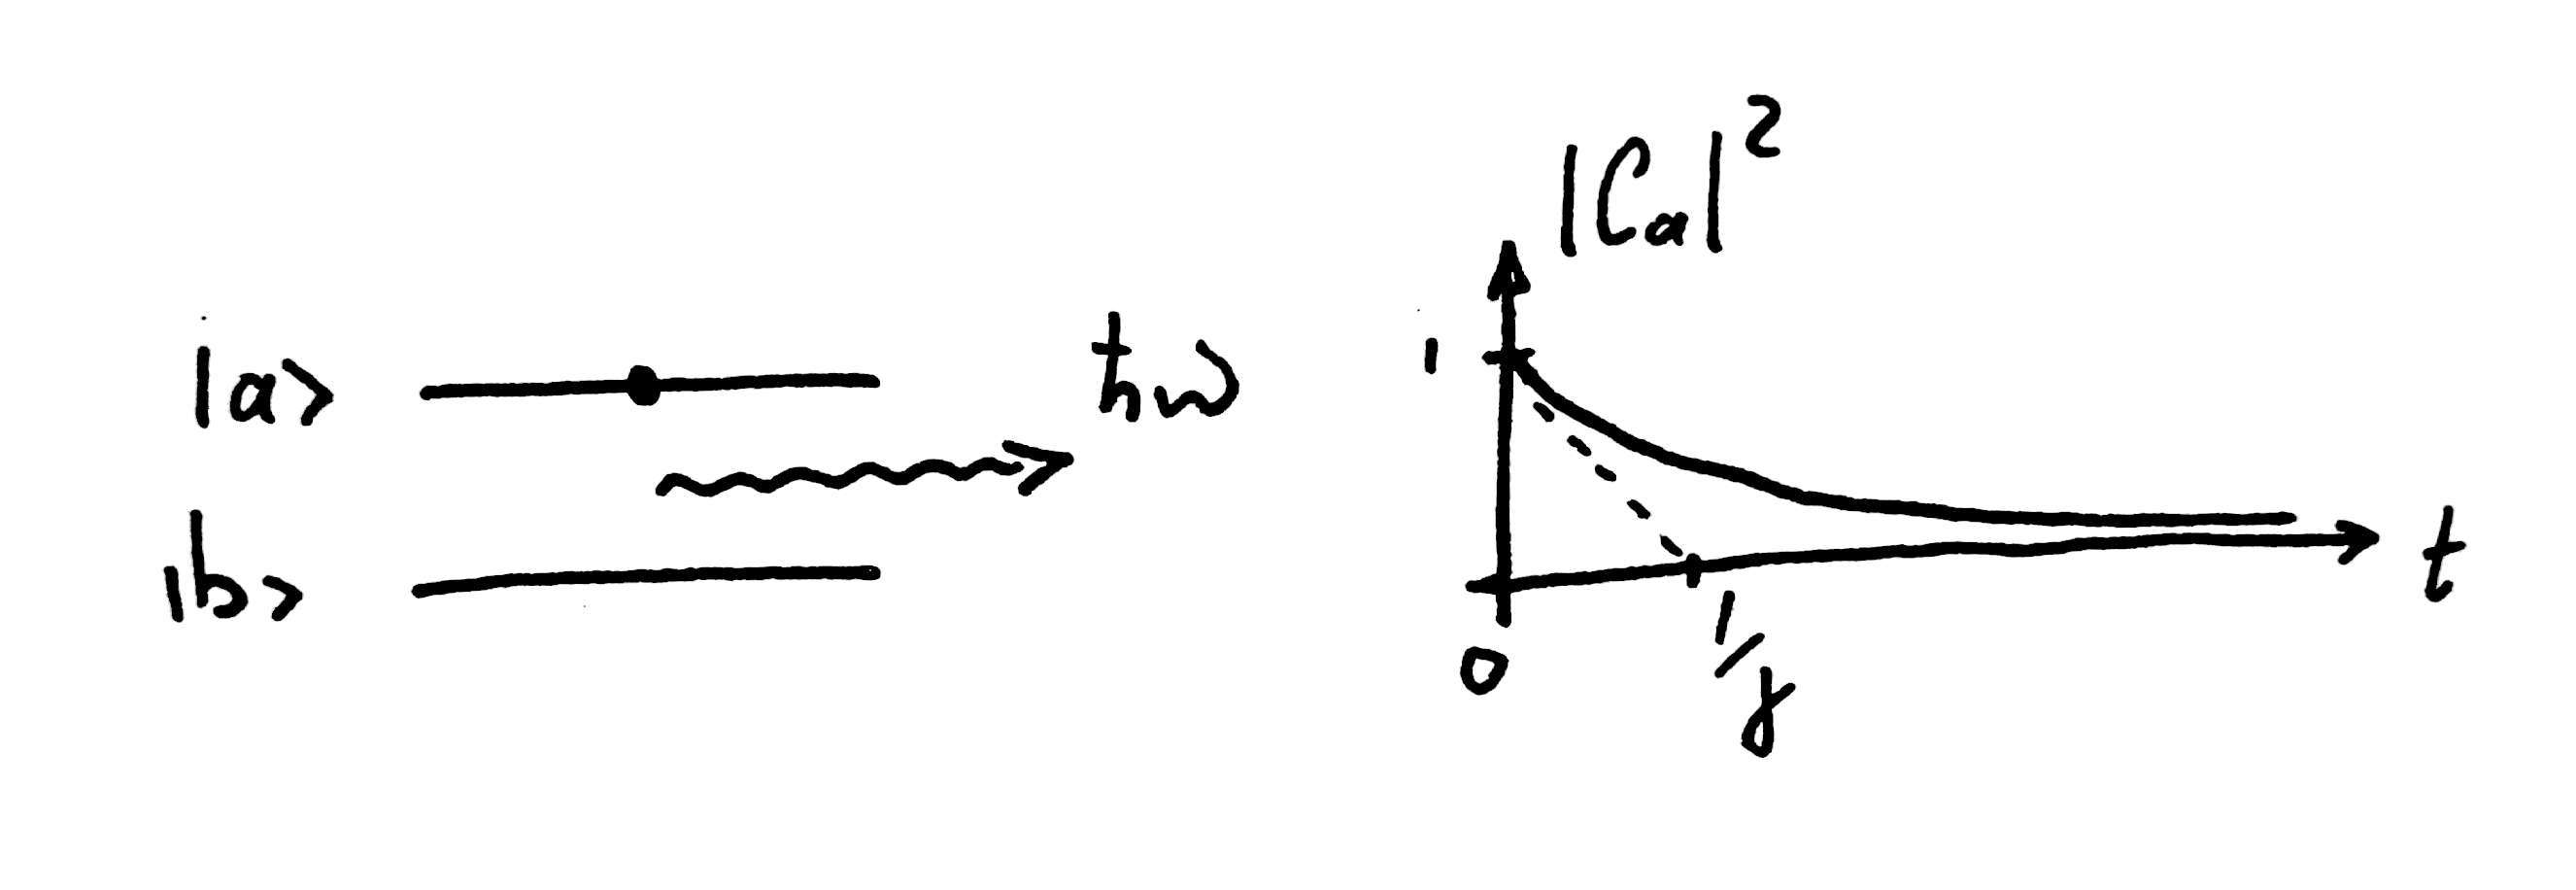
\includegraphics[width=0.65\linewidth]{fig/L7/emissions}
	\caption{Relaxation process}
	\label{fig:emission}
\end{figure}

It is useful to remember that $\gamma \sim n |\vec{d}|^2$ and expression for $\gamma$ contains the Plank constant $\hbar$ which means that this process has a quantum nature.

\textit{Remark:} idea of moves such
\begin{equation}
	\sum_{\kv} \quad \to \quad \int d \omega_{\kv} \quad \to \quad \delta(t - \tau)
\end{equation}
is called the Weisskopf-Wigner method.

In order to compare, when we had a two--level system and a one--mode field we obtained Rabi osculations. In contrast to this, the continuum of modes gives us a relaxation process. 